\documentclass[a4paper]{article}

%% Language and font encodings
\usepackage[dutch]{babel}
\usepackage[utf8x]{inputenc}
\usepackage[T1]{fontenc}
\usepackage{graphicx}
\usepackage{subcaption}

%% Sets page size and margins
\usepackage[a4paper,top=3cm,bottom=3cm,left=3cm,right=3cm,marginparwidth=1.75cm]{geometry}

%% Useful packages
\usepackage{amsmath}

\title{Verzameling oud-examenvragen}
\author{Achim Vandierendonck}
\date{}

\begin{document}
\maketitle

\section*{Vraag 1 (6 punten)}
Beschouw een zeer goede thermische geleider ($k \approx \infty$) in de vorm van een cilinder met lengte $L$ en straal $a_1$. Rond deze geleider zit een cilindrische mantel met dezelfde lengte en straal $a_2$, bestaande uit een materiaal met thermische geleidingscoëfficiënt $k$. De kern is eveneens een (niet-oneindig goede) elektrische geleider, waarover een dc-spanning $V$ staat en waardoor een dc-stroom $I$ loopt. De mantel wordt langs de buitenkant convectief gekoeld (convectiecoëfficiënt $h$). De warmteafvoer langs de twee platte zijvlakken is te verwaarlozen.

\begin{figure}[ht]
    \centering
    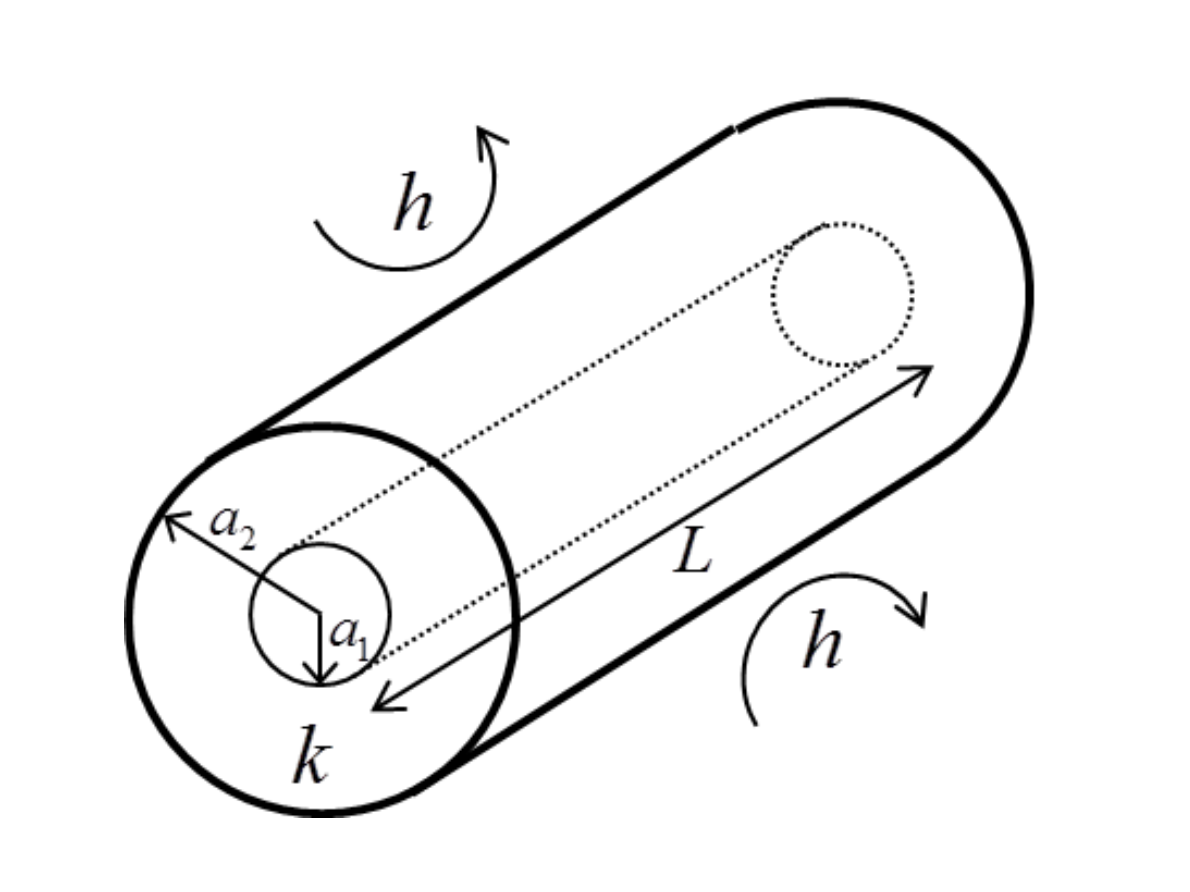
\includegraphics[width=0.5\textwidth]{vraag1}
    \caption{Opstelling van vraag 1}
    \label{fig:vraag1}
\end{figure}

\paragraph{Vraag 1a (2 punten)}
Schrijf de relevante differentiaalvergelijking en randvoorwaarden voor het thermische probleem op.

\paragraph{Vraag 1b (2 punten)}
Hoeveel hoger dan omgevingstemperatuur is de temperatuur aan de buitenkant van de mantel (uitgedrukt als een functie van de gegeven grootheden)?

\paragraph{Vraag 1c (2 punten)}
Wat is de equivalente thermische weerstand voor de geleider (uitgedrukt als een functie van de gegeven grootheden)?

\section*{Vraag 2 (5 punten)}
Twee (oneindig lange) rechthoekige platen (die zich gedragen als Lambertiaanse stralers) wisselen enkel warmte uit door straling. De structuur wordt beschreven in figuur \ref{fig:vraag2}, die oneindig uitgestrekt is in de richting loodrecht op het vlak van de figuur.

\begin{figure}[ht]
    \centering
    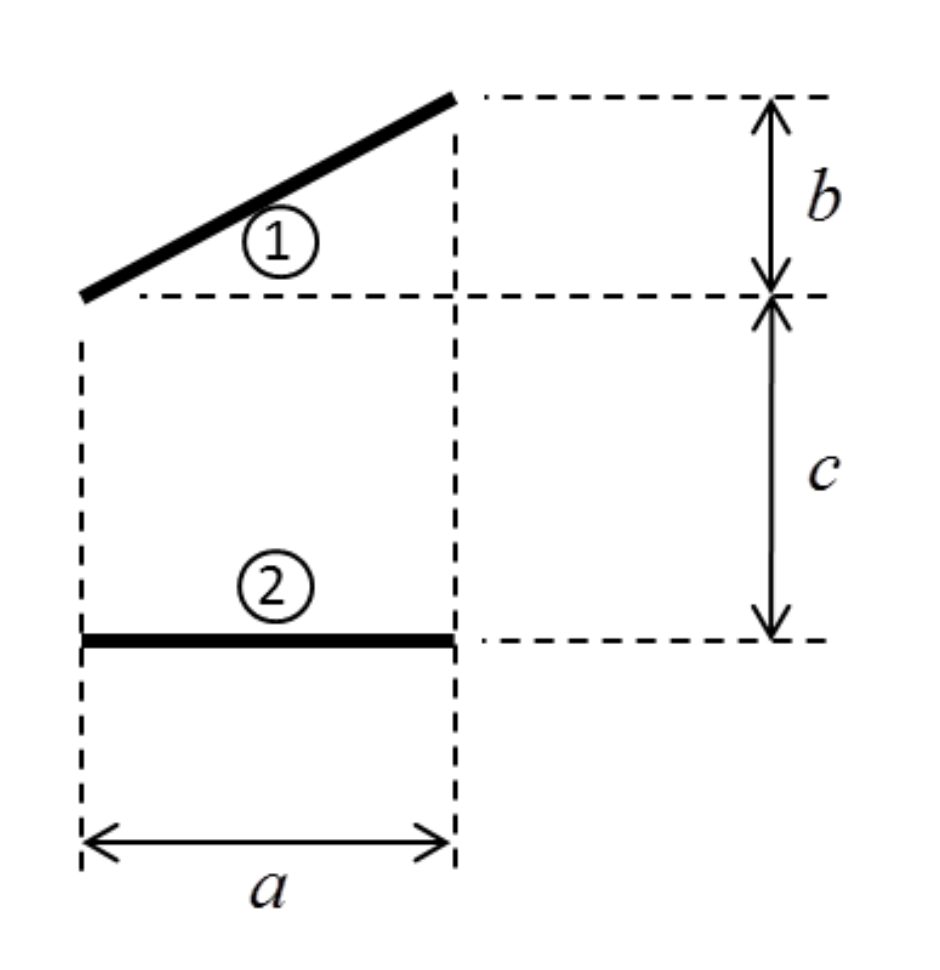
\includegraphics[width=0.5\textwidth]{vraag2}
    \caption{Opstelling van vraag 2}
    \label{fig:vraag2}
\end{figure}

\paragraph{Vraag 2a (2 punten)}
Wat is de geometriefactor voor warmtestraling van oppervlak 1 naar oppervlak 2 (waarbij als oppervlak slechts één kant van de platen bedoeld wordt, de andere kant wordt perfect geïsoleerd verondersteld).

\paragraph{Vraag 2b (1 punt)}
Wat is de geometriefactor voor warmtestraling van oppervlak 2 naar de omgeving (dus naar overal behalve naar oppervlak 1)?

\paragraph{Vraag 2c (2 punten)}
Stel: oppervlak 1 is een warmtebron, waardoor er een klein temperatuursverschil $\Delta T_1$ is tussen de plaat en de omgeving (die zich op kamertemperatuur bevindt).
Wat is dan het temperatuursverschil $\Delta T_2$ tussen oppervlak 2 en de omgeving?

\section*{Vraag 3 (5 punten)}
Een koelvin bestaat uit 6 identieke platen met dikte $d$, breedte $b$ en lengte $a$ (met $d \ll b$
en $d \ll a$), die een structuur vormen zoals in figuur \ref{fig:vraag3}. De koelvin is gemaakt uit een materiaal met thermische geleidingscoëfficiënt $k$, en wordt langs alle brede zijvlakken convectief gekoeld (convectiecoëfficiënt $h$). De warmte-afvoer langs de smalle zijvlakken is te verwaarlozen. In het midden van de koelvin bevindt zich een warmtebron (het gearceerde oppervlak met breedte $b$ en dikte $d$) die een dc-vermogen $P$ (in Watt) dissipeert.

\begin{figure}[ht]
    \centering
    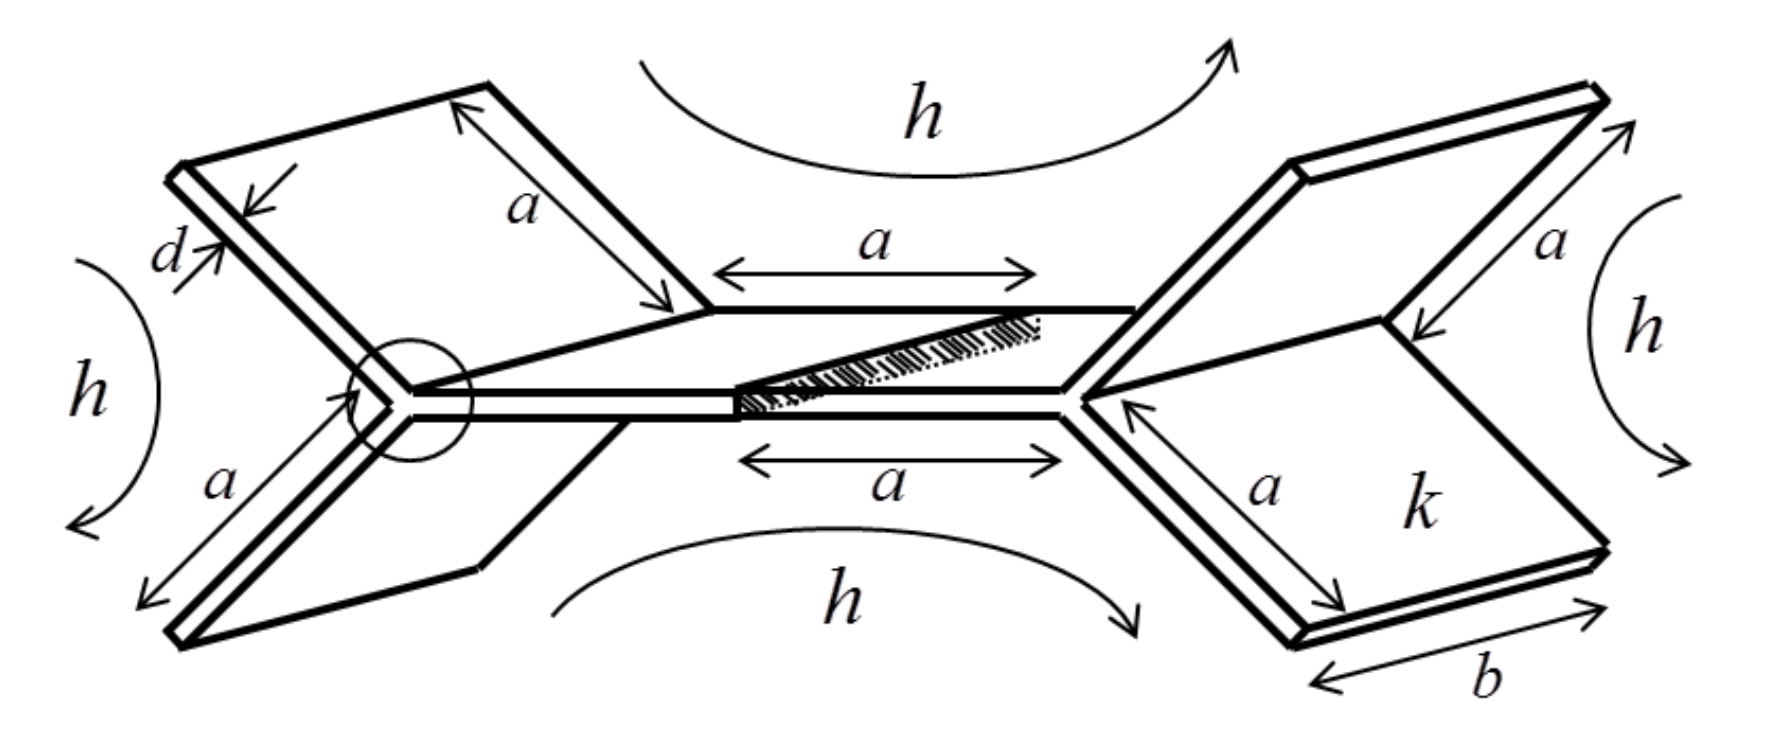
\includegraphics[width=0.5\textwidth]{vraag3}
    \caption{Opstelling van vraag 3}
    \label{fig:vraag3}
\end{figure}

\paragraph{Vraag 3a (2 punten)}
Teken een equivalent elektrisch netwerk en druk de netwerkelementen uit in functie van de gegeven grootheden. Voor volgende vragen mag je het resultaat van deze vraag gekend veronderstellen (je moet de netwerkelementen dus niet opnieuw expliciet uitschrijven).

\paragraph{Vraag 3b (2 punten)}
Wat is de equivalente thermische weerstand van de warmtebron?

\paragraph{Vraag 3c (1 punt)}
Wat is de temperatuur op de “vertakkingspunten” van de koelvin (aangeduid met een cirkeltje op de figuur)?

\section*{Vraag 4 (4 punten)}
Beschouw onderstaande figuur: een achtste van de ruimte (waarvan de zijvlakken loodrecht op elkaar staan) met daaruit weggenomen een achtste van een bol met straal $a$, bestaat uit een materiaal met thermische geleidingscoëfficiënt $k$ en specifieke warmte $C_V$. Op het ronde oppervlak bevindt zich een warmtebron die een vermogen dissipeert waarvan het tijdsafhankelijke gedeelte gelijk is aan $P_0\cos{\omega t}$ (in Watt). Alle wanden zijn perfect isolerend.

\noindent Wat is de temperatuur in functie van de positie en de tijd in het materiaal?

\begin{figure}[ht]
    \centering
    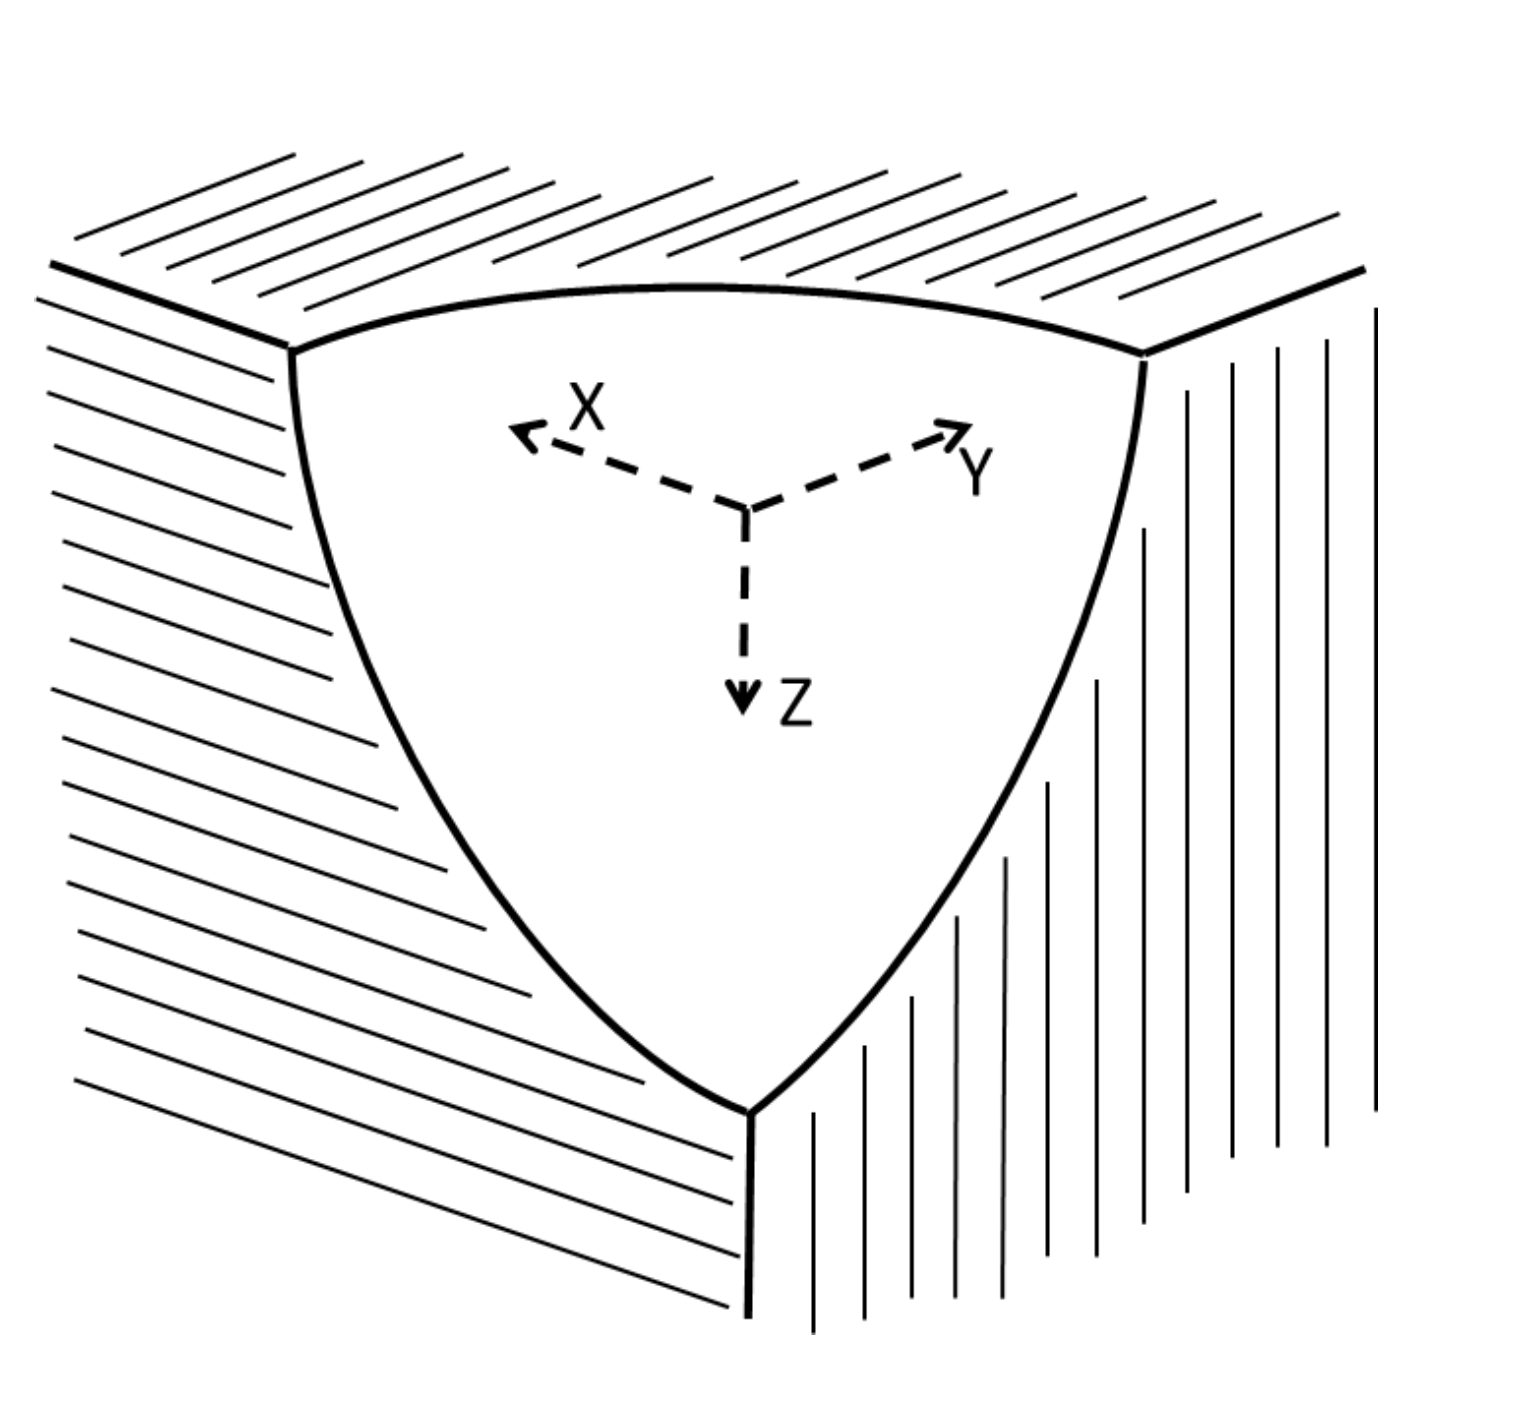
\includegraphics[width=0.5\textwidth]{vraag4}
    \caption{Opstelling van vraag 4}
    \label{fig:vraag4}
\end{figure}

\section*{Vraag 5 (4 punten)}
Door een (bij benadering oneindig lange) cilindervormige buis met straal $R$ stroomt een vloeistof met dichtheid $\rho$, viscositeit $\mu$, warmtegeleidingscoëfficiënt $k$ en specifieke warmte $C_V$. In het midden van de buis wordt de snelheid van de vloeistof op $v_0$ gehouden.

\paragraph{Vraag 5a (1 punt)}
Schrijf de relevante differentiaalvergelijkingen en randvoorwaarden op om de vloeistofsnelheid overal in de buis te berekenen.

\paragraph{Vraag 5b (1 punt)}
Bereken de vloeistofsnelheid overal in de buis.

\paragraph{Vraag 5c (1 punt)}
Welk drukverschil (per lengte-eenheid) is nodig om deze snelheid te onderhouden?

\paragraph{Vraag 5d (1 punt)}
Stel dat de temperatuurverdeling voor deze vloeistof in de buis gekend is. We willen willen nu een vloeistof gebruiken met een specifieke warmte die maar half zo groot is: $C_V' = C_V/2$, maar wel dezelfde temperatuursverdeling behouden. Hoe moeten we dan de aanstroomsnelheid aanpassen?


\section*{Vraag 6 (4 punten)}
Twee (oneindig lange) rechthoekige platen (die zich gedragen als Lambertiaanse zwarte stralers) wisselen enkel warmte uit door straling. De structuur wordt beschreven in figuur \ref{fig:vraag6}, die oneindig lang uitgestrekt is in de richting loodrecht op het vlak van de figuur.

\begin{figure}[ht]
    \centering
    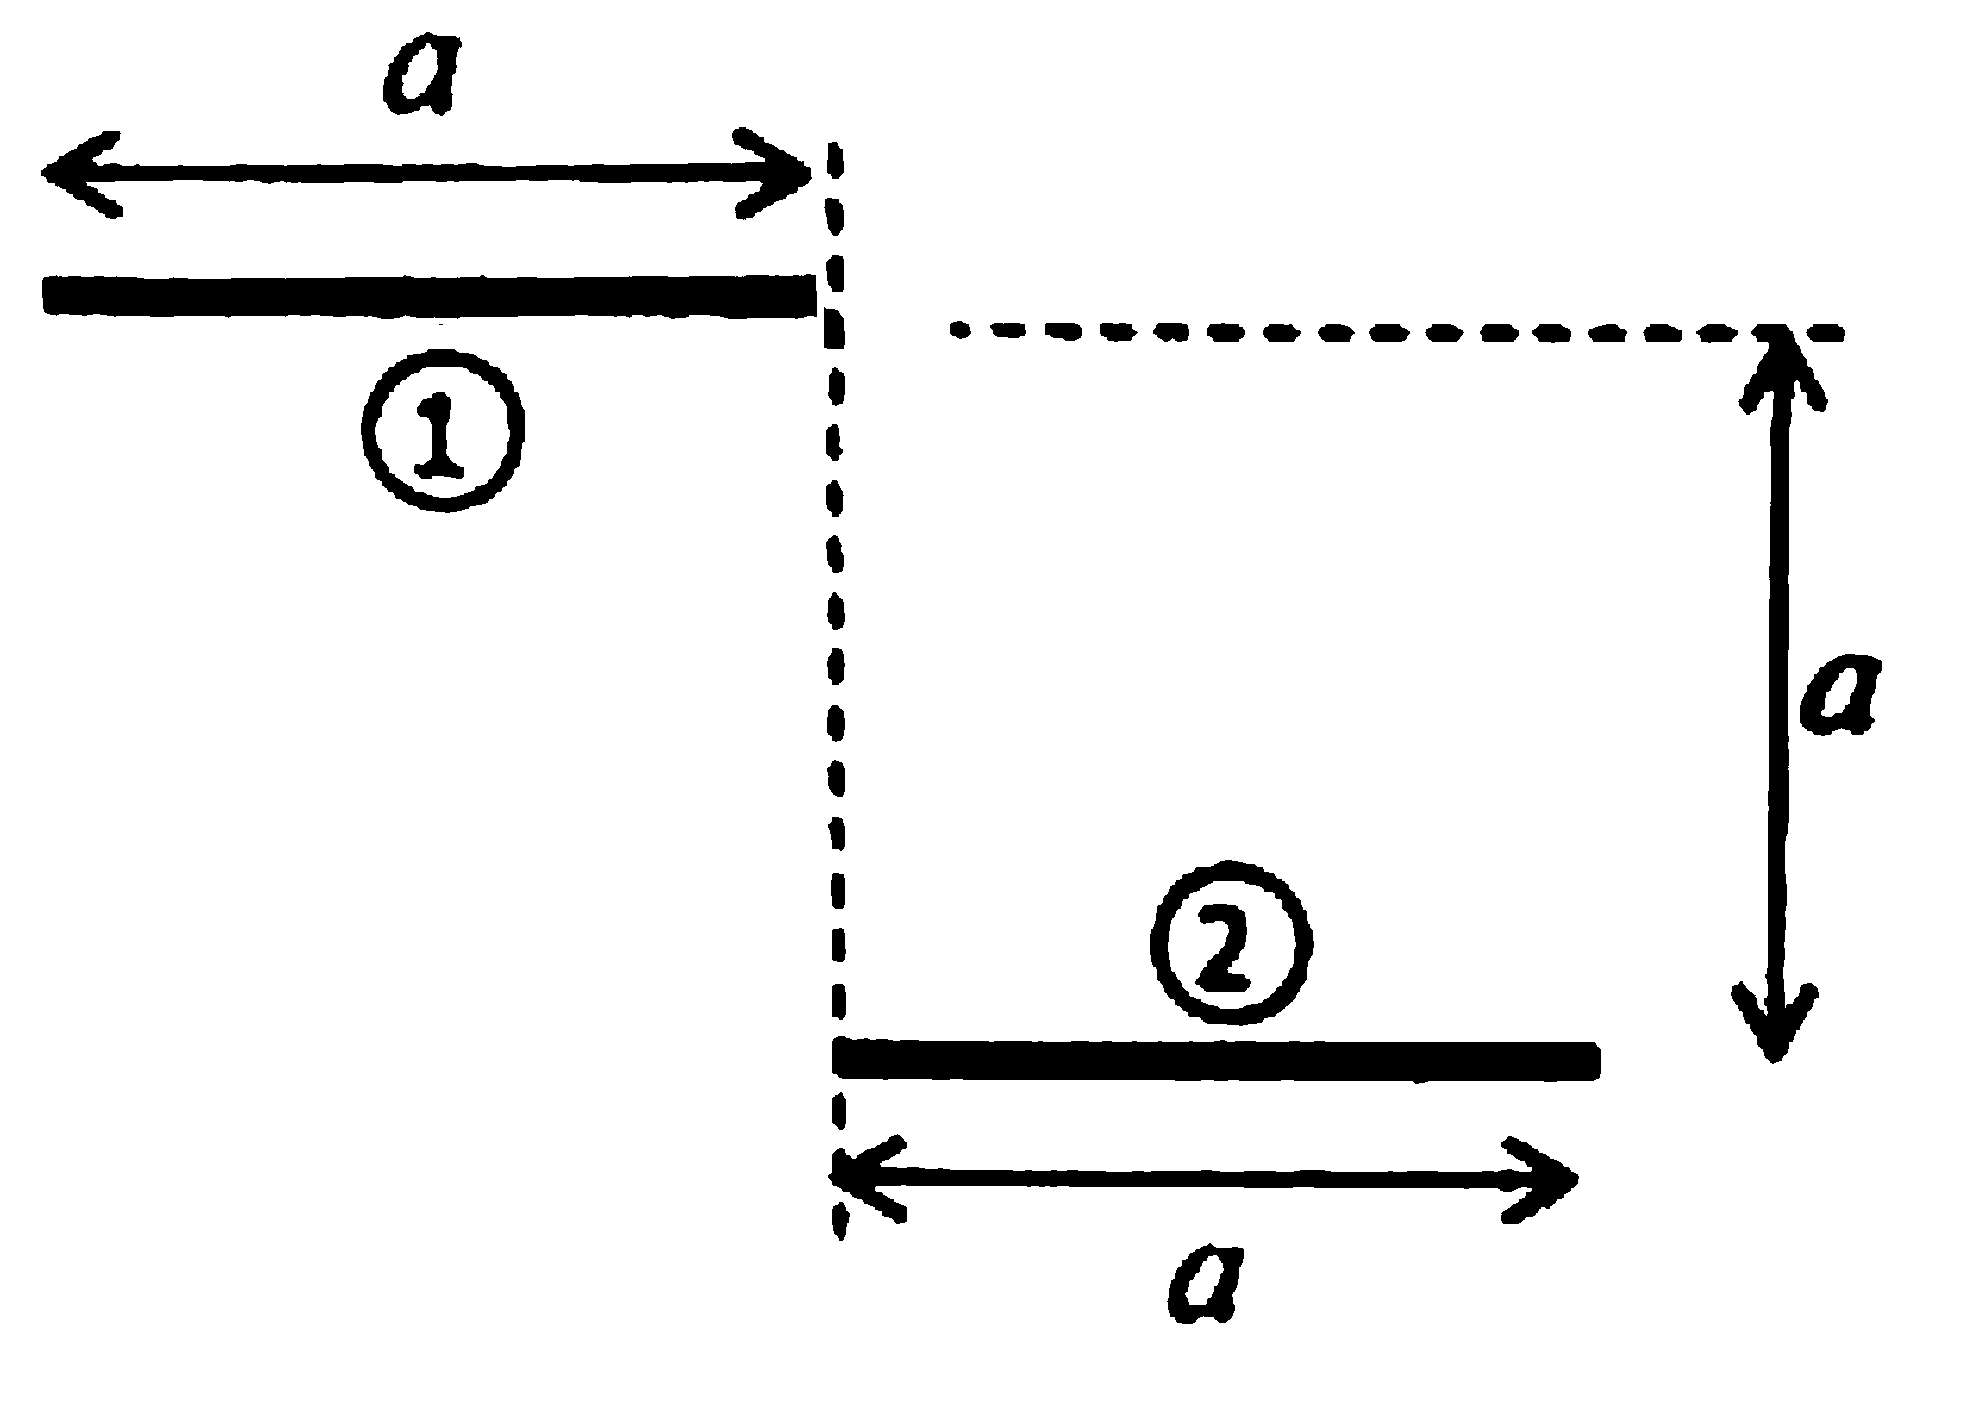
\includegraphics[width=0.5\textwidth]{vraag6}
    \caption{Opstelling van vraag 6}
    \label{fig:vraag6}
\end{figure}

\paragraph{Vraag 6a (2 punten)}
Wat is de geometriefactor voor de warmtestraling van oppervlak 2 naar oppervlak 1 (waarbij als oppervlak slechts één kant van de platen bedoeld wordt, de andere kant wordt perfect geïsoleerd verondersteld).

\paragraph{Vraag 6b (6 punt)}
Wat is de geometriefactor voor de warmtestraling van oppervlak 1 naar de omgeving (dus naar overal behalve naar oppervlak 2).

\paragraph{Vraag 6c (6 punt)}
Stel: oppervlak 1 is een warmtebron, waardoor er een kleine temperatuursverschil $\Delta T_1$ is tussen de plaat en de omgeving (die zich op kamertemperatuur bevindt). Wat is dan het temperatuursverschil $\Delta T_2$ tussen oppervlak 2 en de omgeving.

\section*{Vraag 7 (4 punten)}
Beschouw een kubus met zijde $a$, bestaande uit een materiaal met thermische geleidingscoëfficiënt $k$ en specifieke warmte $C_V$. Het onderste vlak van de kubus is een homogene elektrische weerstand met weerstandswaarde $R$, waarover een sinusoïdale spanning $V = V_0\cos{\omega t}$ wordt aangelegd. Het bovenste vlak van de kubus wordt op omgevingstemperatuur gehouden. Alle vlakken behalve het bovenste zijn geïsoleerd.

\paragraph{Vraag 7a (1 punt)}
Geef aan hoe het probleem vereenvoudigd kan worden door gebruik te maken van superpositie, beeldwarmtebronnen, etc.

\paragraph{Vraag 7b (1 punt)}
Schrijf de relevante differentiaalvergelijking(en) en randvoorwaarden op die samen de vereenvoudigingen uit 7a tot een oplossing kunnen leiden.

\paragraph{Vraag 7c (1 punt)}
Bereken de temperatuursverdeling in de kubus, in het frequentiedomein.

\paragraph{Vraag 7d (1 punt)}
Geef een uitdruking voor de temperatuursverdeling in de kubus in het tijdsdomein.

\section*{Vraag 8 (4 punten)}
Beschouw een plaat die zich oneindig uitstrekt in 2 dimensies. De plaat bestaat uit verschillende lagen (zie figuur \ref{fig:vraag81} van links naar rechts):
\begin{itemize}
    \item Een homogeen verdeelde warmtebron die een vermogen $p$ per oppervlakte-eenheid dissipeert.
    \item Een warmtegeleidende laag, met dikte $d$, en thermische conductiviteit $k$.
    \item Een oneindig dunne grenslaag, die je perfect warmtegeleidend mag veronderstellen.
    \item Een laag, met dikte $d$, met daarin vacuum.
    \item Een oneindig dunne, perfect warmtegeleidende plaat, met daarin gaten op regelmatige afstand van elkaar (zie figuur \ref{fig:vraag82}). De afstand tussen de gaten is $b$, de straal is $a$.
    \item Opnieuw een laag, met dikte $d$, met daarin vacuum.
    \item Een oneindig dunne, perfect warmtegeleidende plaat, die convectief gekoeld wordt met convectiecoëfficiënt $h$.
\end{itemize}

\paragraph{Vraag 8a (1 punt)}
Teken een equivalent elektrisch netwerk.

\paragraph{Vraag 8b (3 punten)}
Wat is de temperatuur van de warmtebron, in functie van $p, k, h, a, b, d,$ etc?

\begin{figure}[ht]
    \centering
    \begin{subfigure}[b]{0.5\textwidth}
        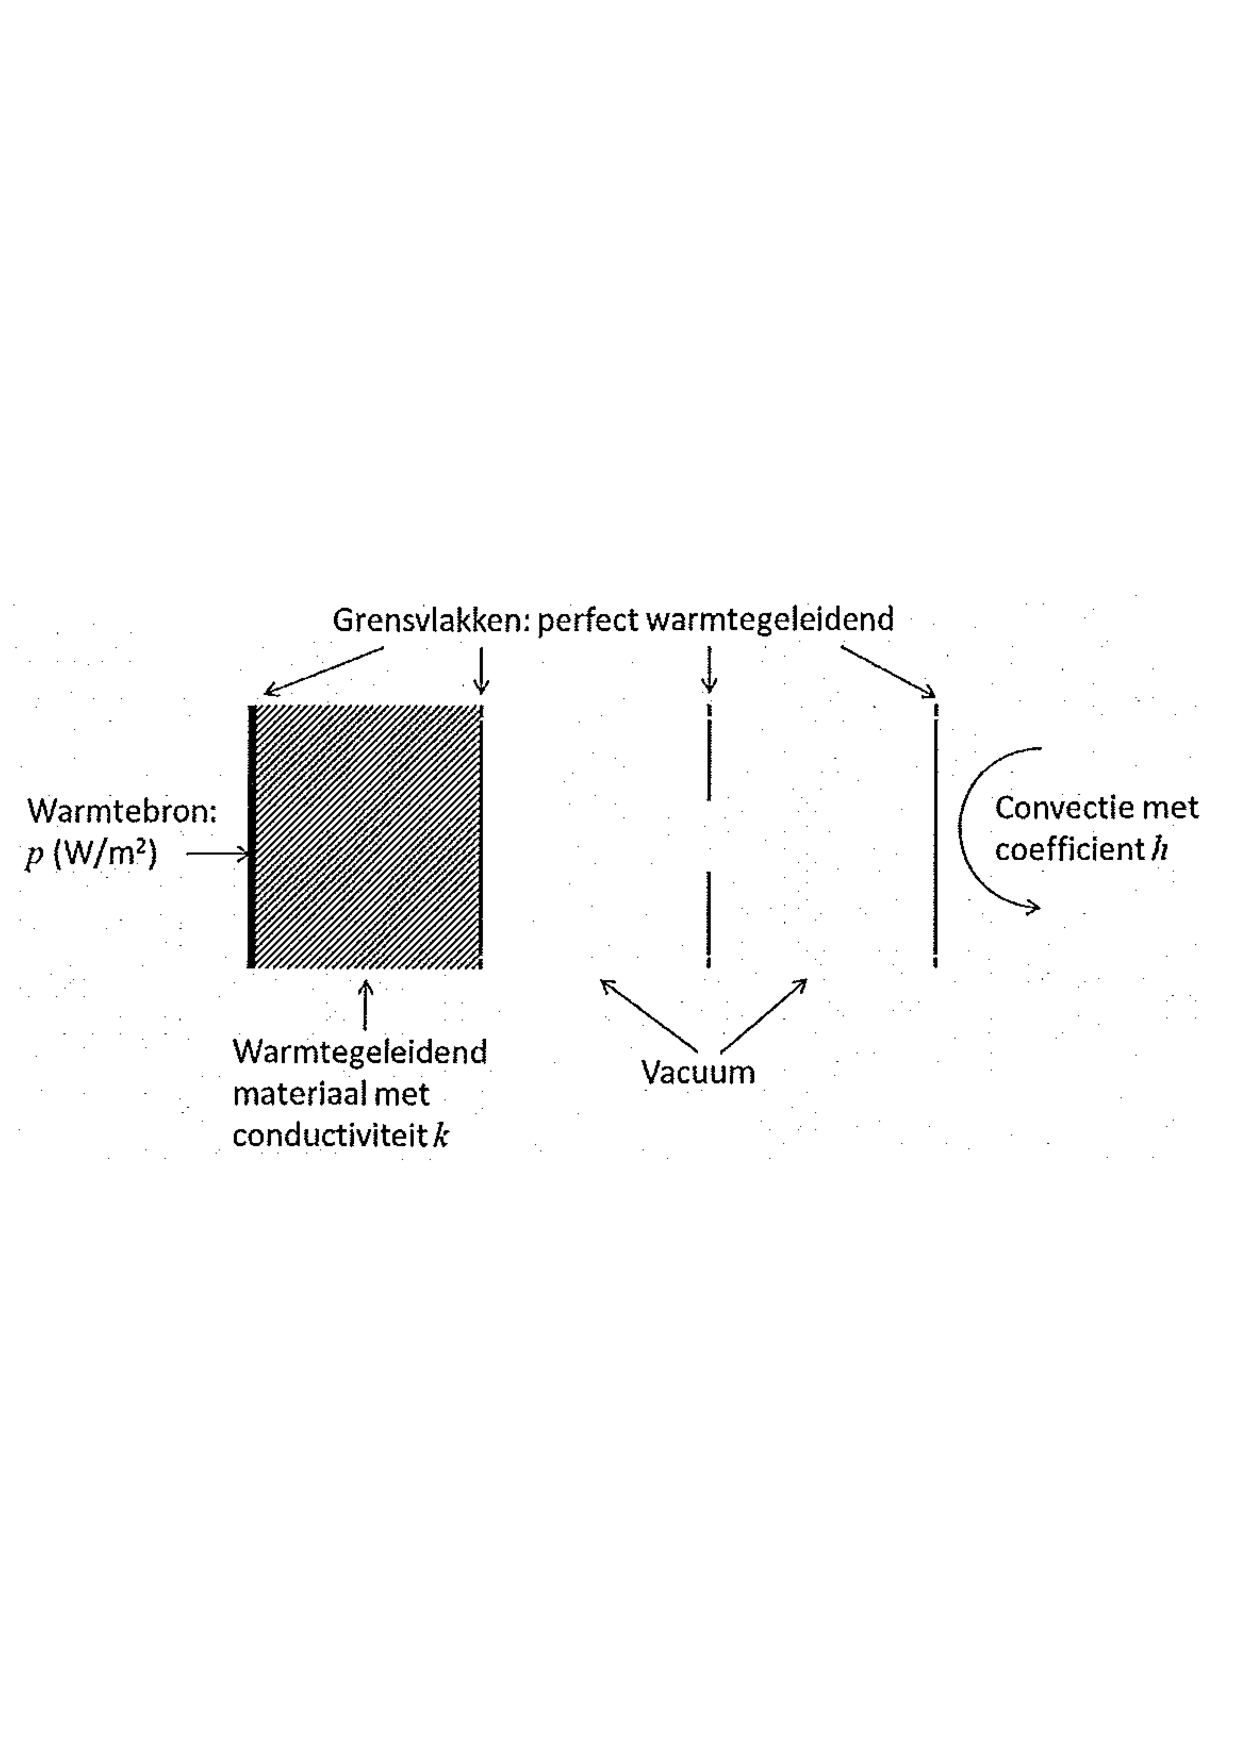
\includegraphics[width=\textwidth]{vraag8-1}
        \caption{Zij-aanzicht}
        \label{fig:vraag81}
    \end{subfigure}%
    \begin{subfigure}[b]{0.5\textwidth}
        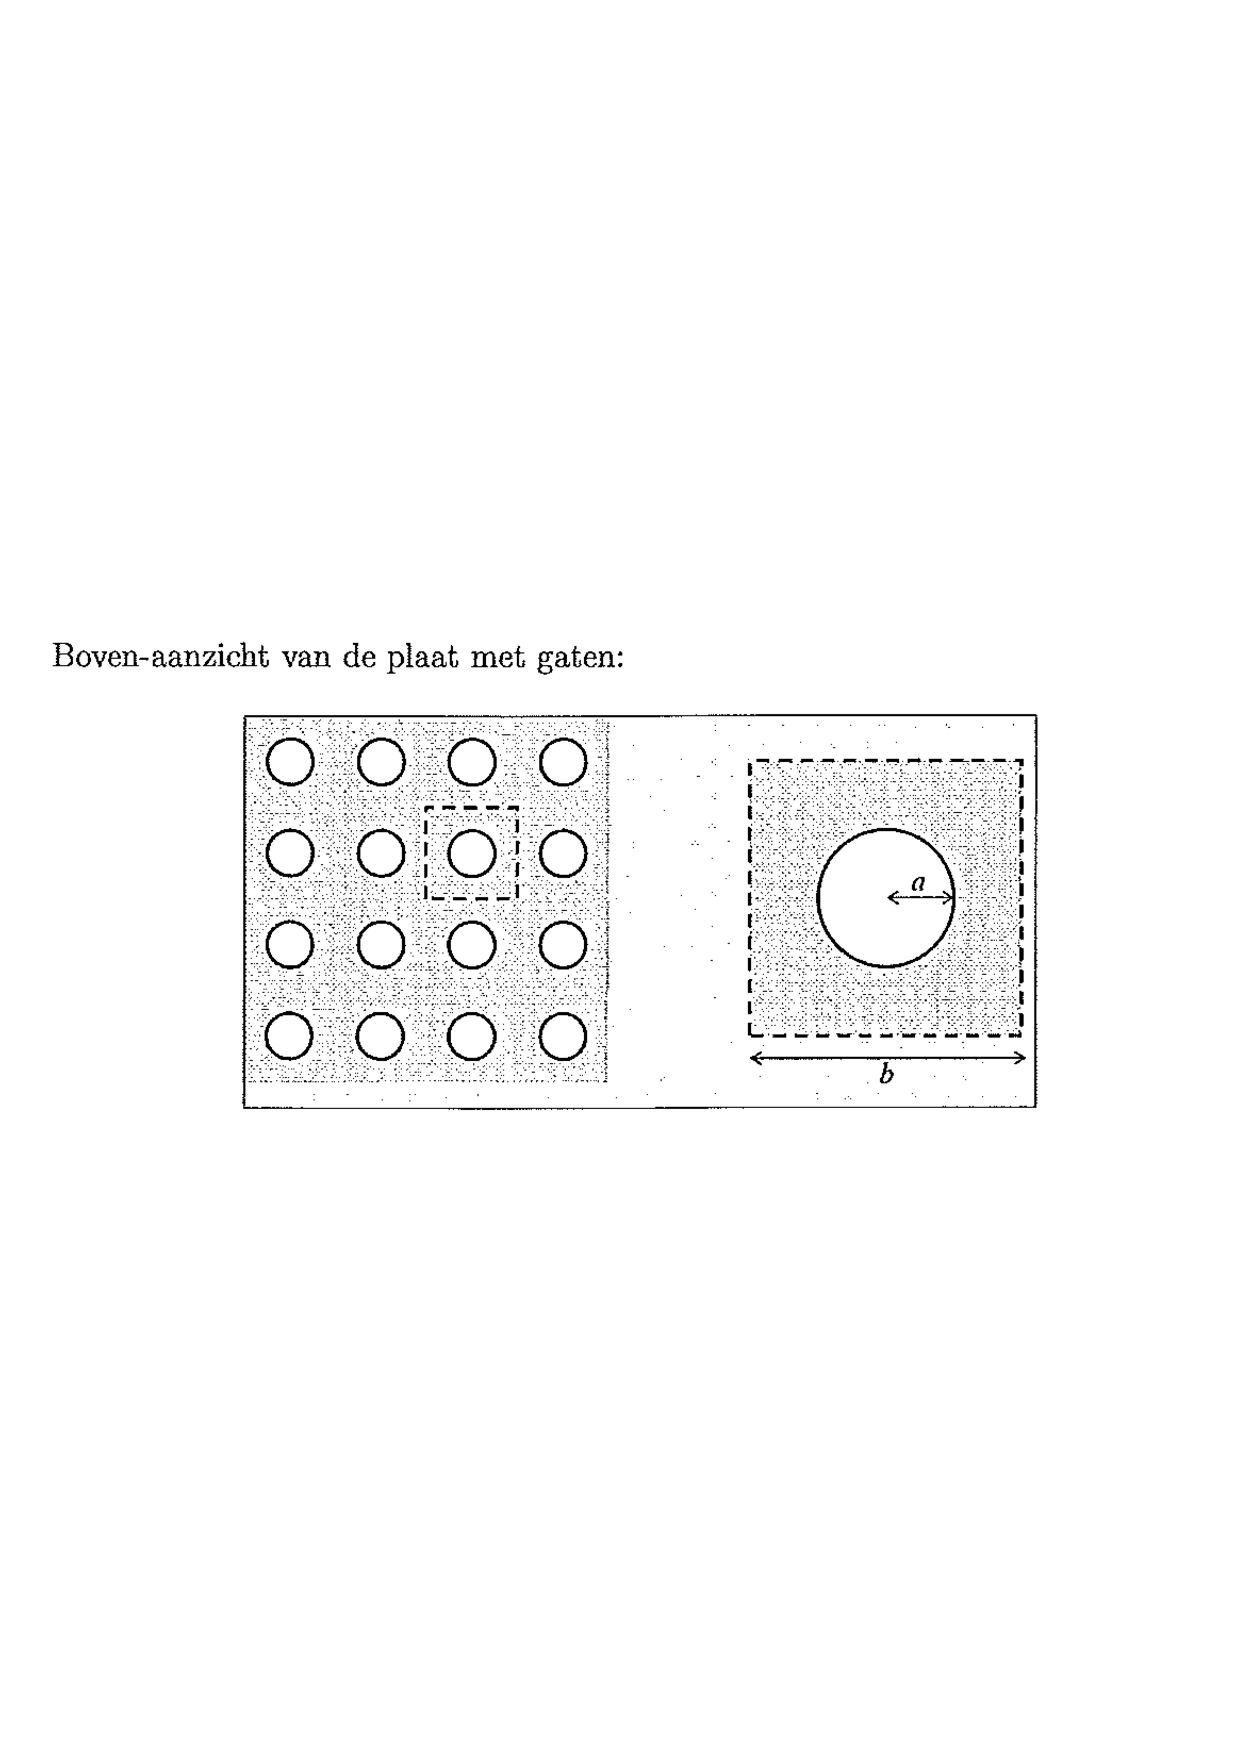
\includegraphics[width=\textwidth]{vraag8-2}
        \caption{Boven-aanzicht}
        \label{fig:vraag82}
    \end{subfigure}
    \caption{Opstelling van vraag 8}
    \label{fig:vraag8}
\end{figure}

\section*{Vraag 9 (4 punten)}
Beschouw een kubus met zijde $a$, bestaande uit een materiaal met thermische geleidingscoëfficiënt $k$ en specifieke warmte $C_V$. Het onderste vlak van de kubus is een warmtebron die op $t = 0$ een impulsvermogen $P$ (in Watt) dissipeert (homogeen over het oppervlak): $P = P_0\delta(t)$. Het bovenste vlak van de kubus wordt op omgevingstemperatuur gehouden. Alle vlakken behalve het bovenste zijn geïsoleerd.

\paragraph{Vraag 9a (1 punt)}
Geef aan hoe het probleem vereenvoudigd kan worden door gebruik te maken van superpositie, beeldwarmtebronnen, etc.

\paragraph{Vraag 9b (1 punt)}
Schrijf de relevante differentiaalvergelijking(en) en randvoorwaarden op die samen de vereenvoudigingen uit 9a tot een oplossing kunnen leiden.

\paragraph{Vraag 9c (1 punt)}
Bereken de temperatuursverdeling in de kubus, in het Laplacedomein.

\paragraph{Vraag 9d (1 punt)}
Geef een uitdruking voor de temperatuursverdeling in de kubus in het tijdsdomein.

\section*{Vraag 10}
Op de kruising van 3 platen (zie figuur \ref{fig:vraag10}, met $d \ll b$ en $d \ll a$), bevindt zich een warmtebron die een vermogen $P$ (in Watt) dissipeert. De platen zijn gemaakt uit een materiaal met thermische geleidingscoëfficiënt $k$, en worden langs alle brede zijvlakken convectief gekoeld (convectiecoëfficiënt $h$). De warmte-afvoer langs de smalle zijvlakken is te verwaarlozen.

\begin{figure}[ht]
    \centering
    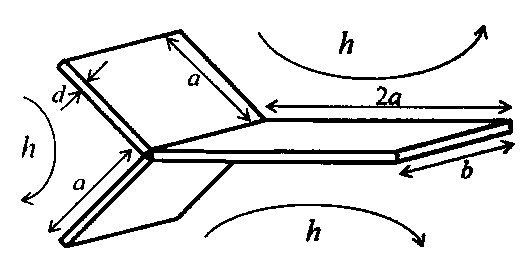
\includegraphics[width=0.5\textwidth]{vraag10}
    \caption{Opstelling van vraag 10}
    \label{fig:vraag10}
\end{figure}

\paragraph{Vraag 10a (1 punt)}
Teken een equivalent elektrisch netwerk en druk de netwerkelementen uit in functie van de gegeven grootheden.

\paragraph{Vraag 10b (1 punt)}
Wat is de equivalente thermische weerstand van de warmtebron?

\paragraph{Vraag 10c (1 punt)}
Schrijf de relevante differentiaalvergelijking en randvoorwaarden op voor de lange plaat.

\paragraph{Vraag 10d (1 punt)}
Bereken de temperatuur in functie van de positie in de lange plaat. Je mag eerder gevonden grootheden gekend veronderstellen (je moet de netwerkelementen dus niet opnieuw expliciet uitschrijven).

\end{document}